%! TEX root = ../../DesignDocument.tex
\hspace{7mm}
The following images show the final Phase One version of the project. 
\subsection{Public Content}
    \hspace{7mm} The Public Content homepage displays all publicly viewable content with options for searching and filtering the table. Clicking on a row will expand the row to reveal options. 
    \label{fig:final_public_content_page}
    \begin{figure}[H]
        \centering 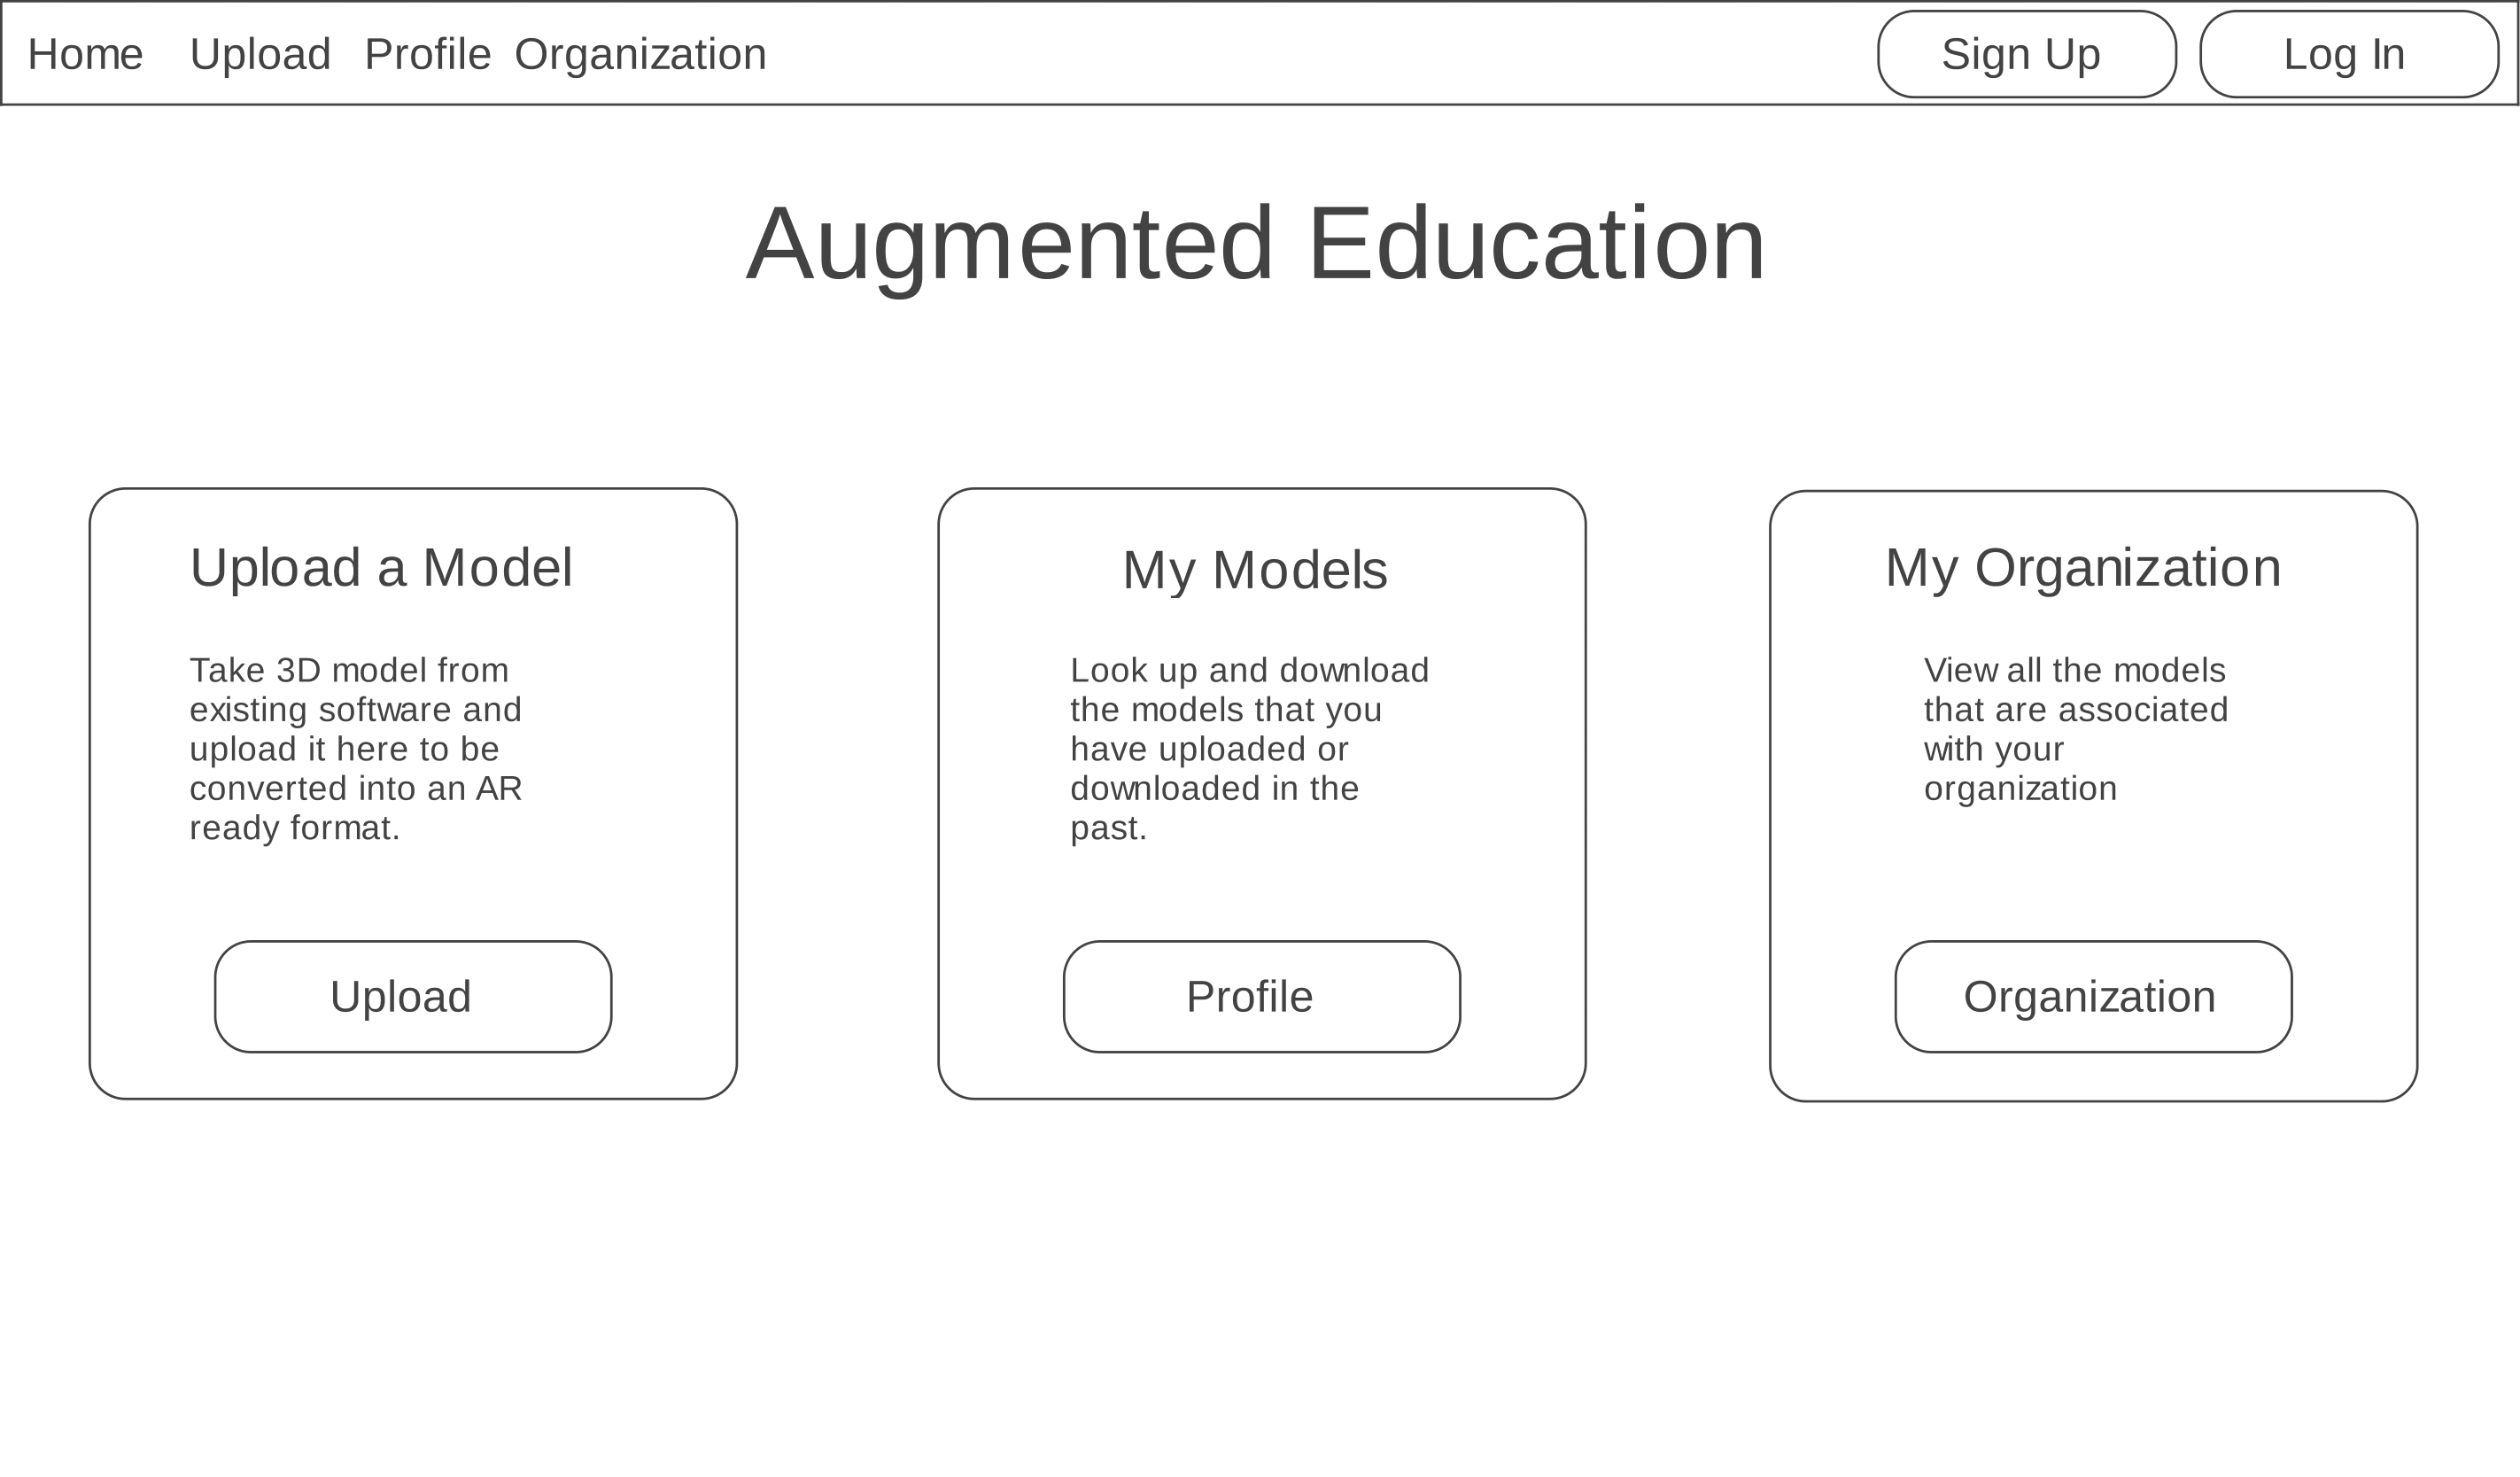
\includegraphics[width=0.6\linewidth]{Home}
        \caption{Final design for the Public Content homepage}
    \end{figure}

\subsection{Upload Page}
    \hspace{7mm} The page where a user can fill out a form 
    that allows them to browse to a 3D model file on their computer and upload
    it to the ASP.NET website under their user account.
    \ \\
    \label{fig:final_upload_page}
    \begin{figure}[H]
        \centering 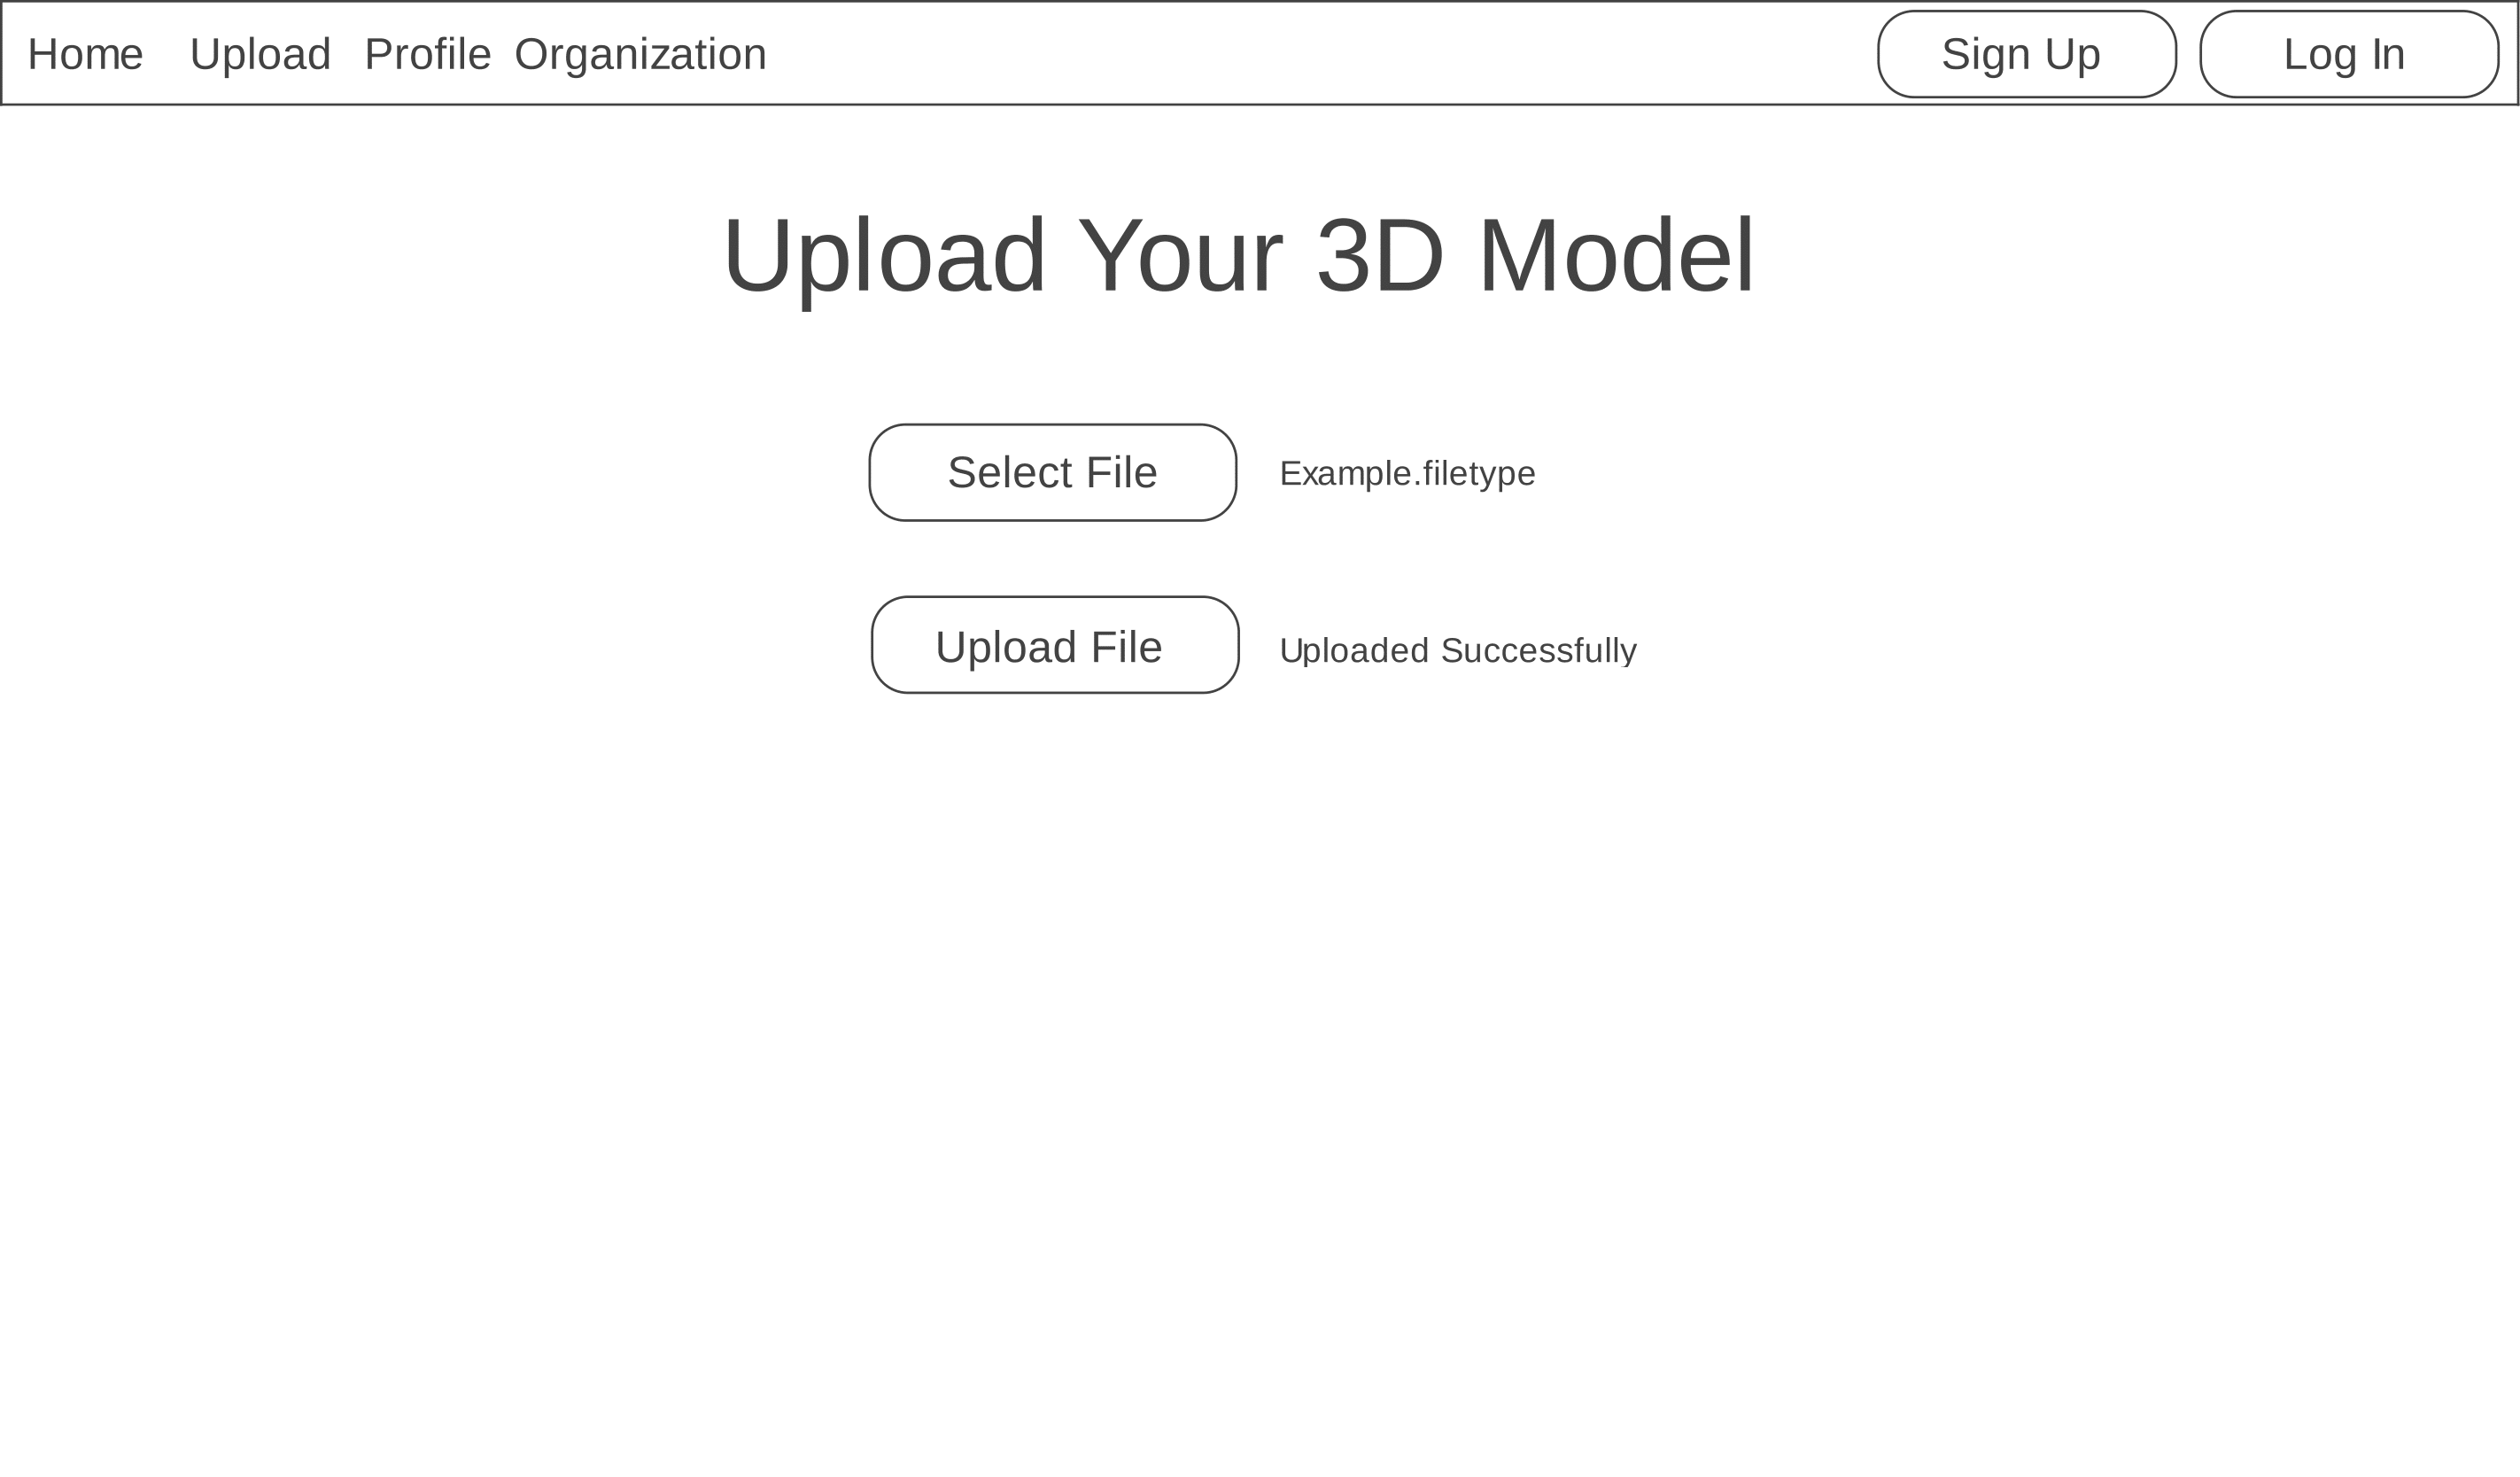
\includegraphics[width=0.6\linewidth]{Upload}
        \caption{Final design for the Upload page}
    \end{figure}

\subsection{My Content}
    \hspace{7mm}
    A page where a user may view all of their public and private files being stored 
    on the cloud.
    \ \\
    \label{fig:final_my_content_page}
    \begin{figure}[H]
        \centering 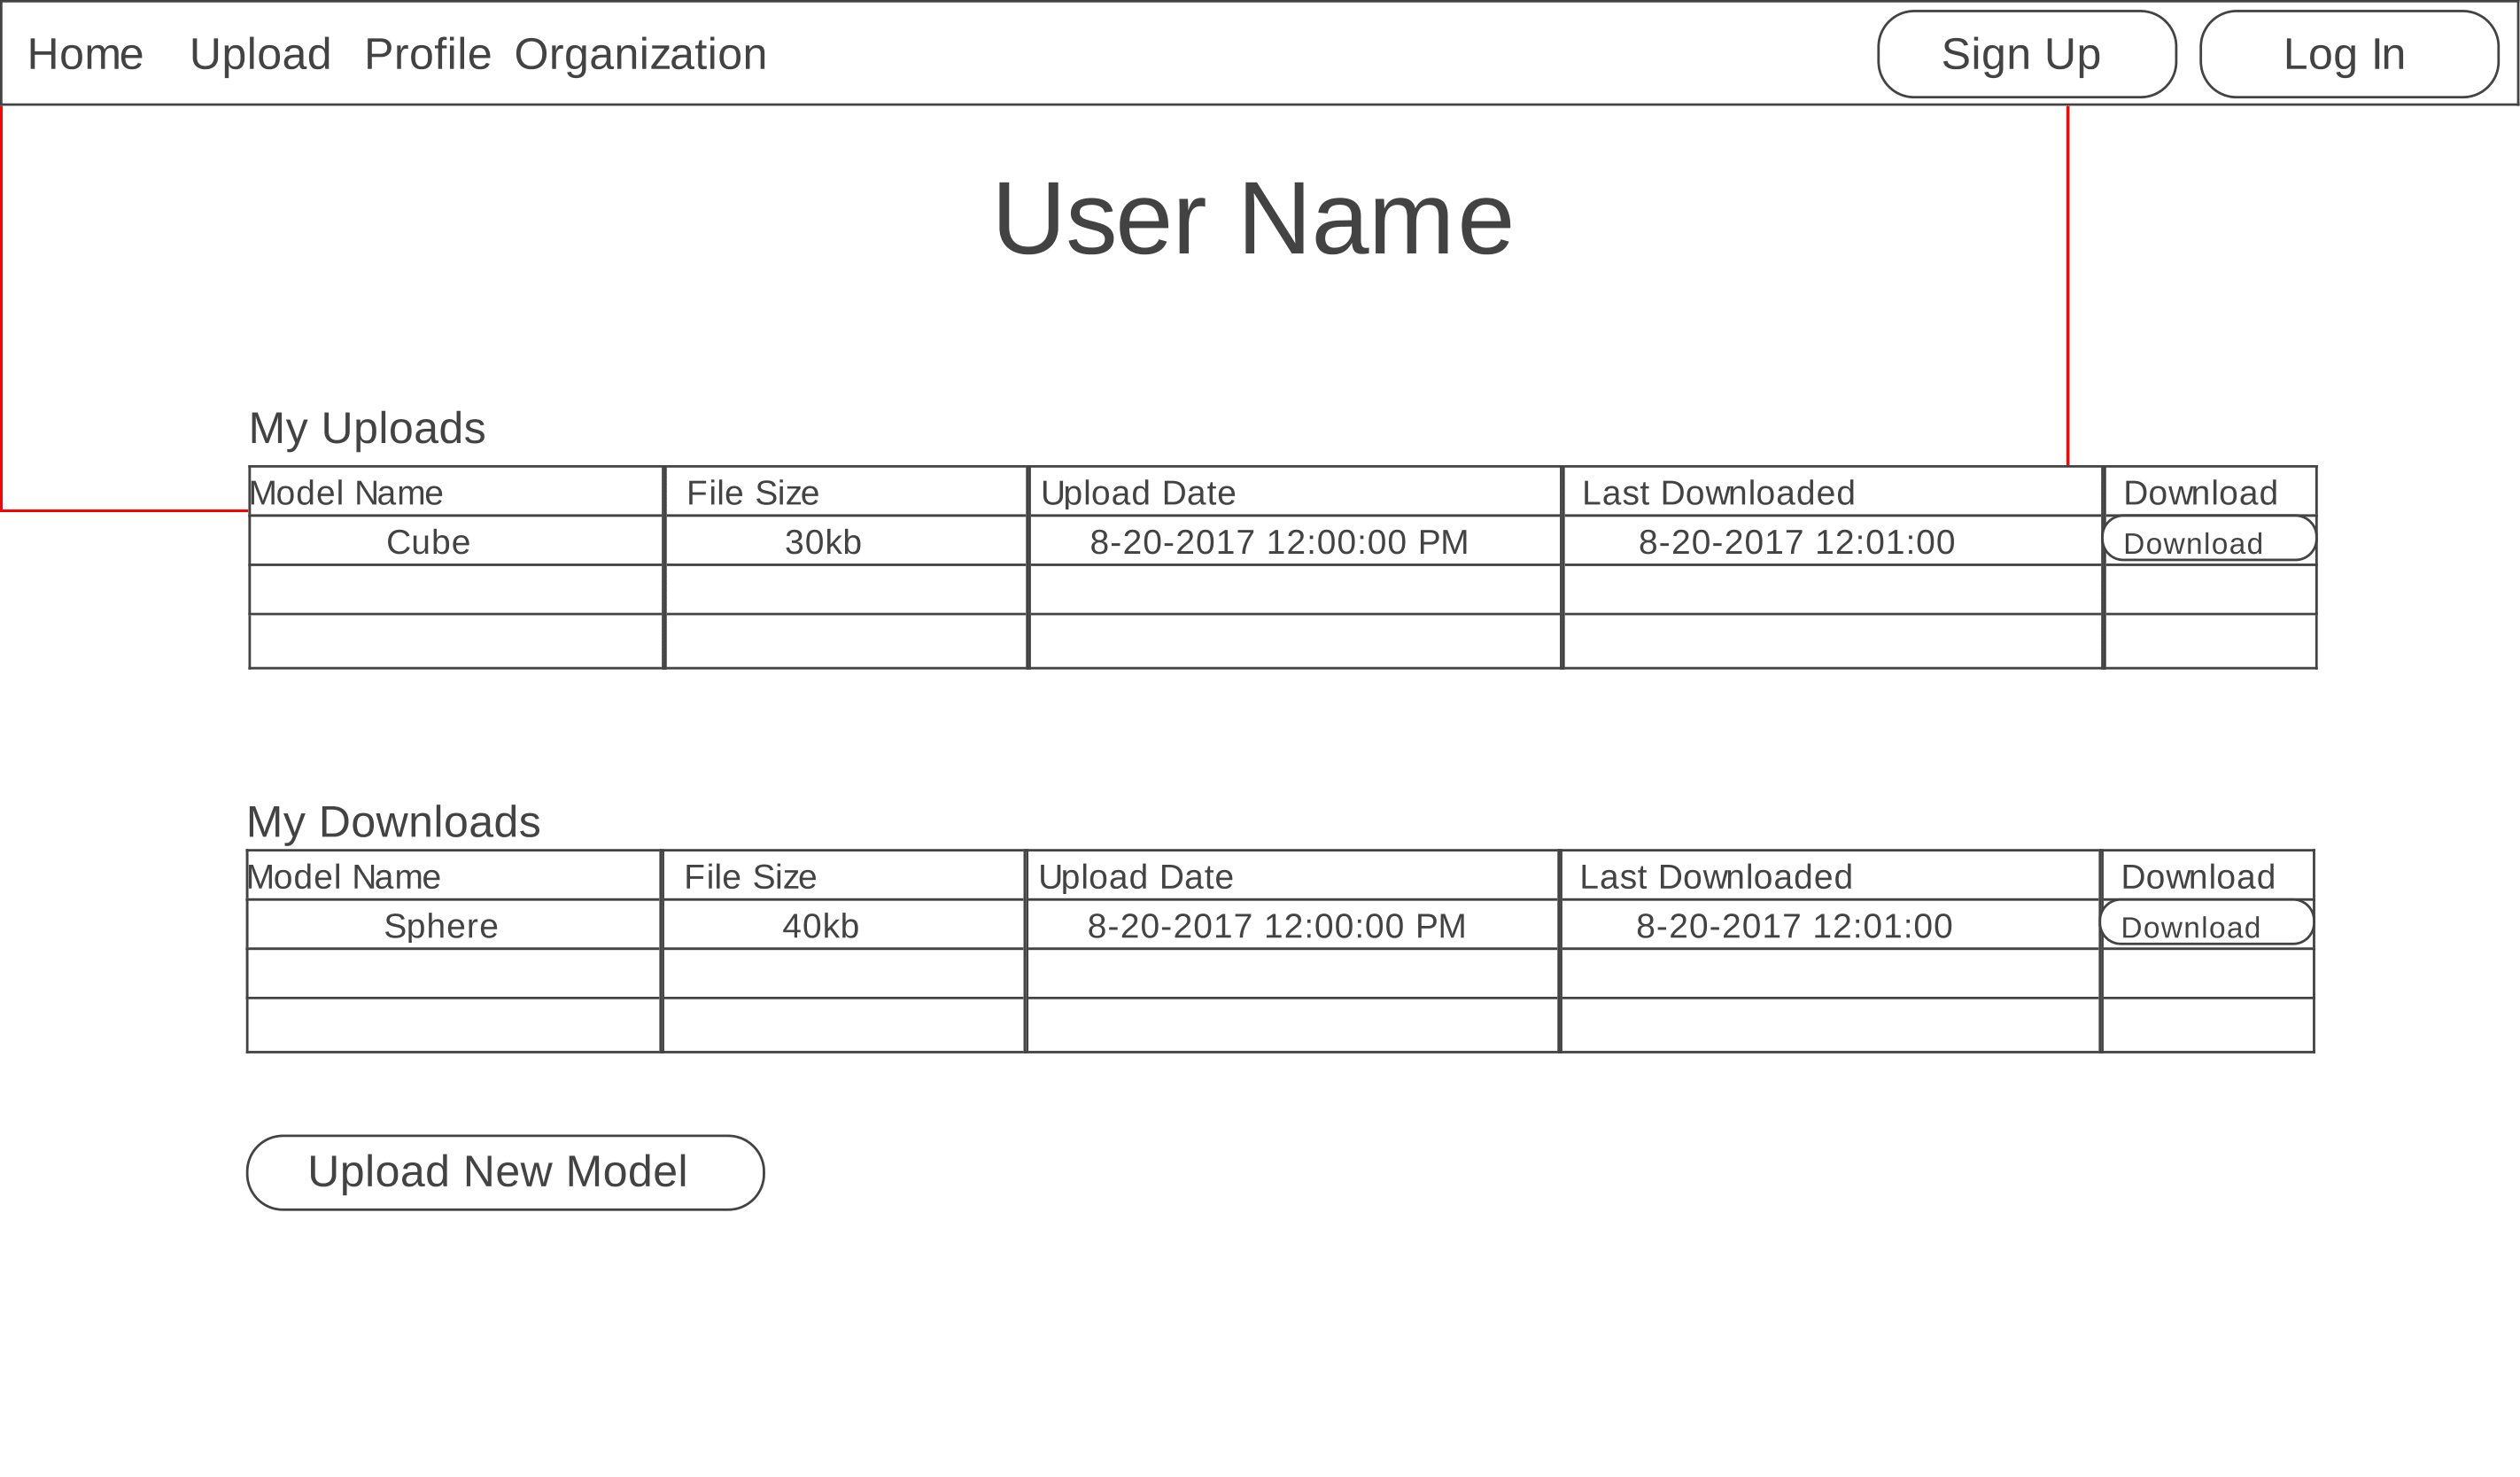
\includegraphics[width=0.6\linewidth]{UserPage}
        \caption{Final design for the My Content page}
    \end{figure}

\subsection{Help Page}
    \hspace{7mm}
    A page displaying simple use instructions for the Augmented Education platform. 
    \ \\
    \label{fig:final_help_page}
    \begin{figure}[H]
        \centering 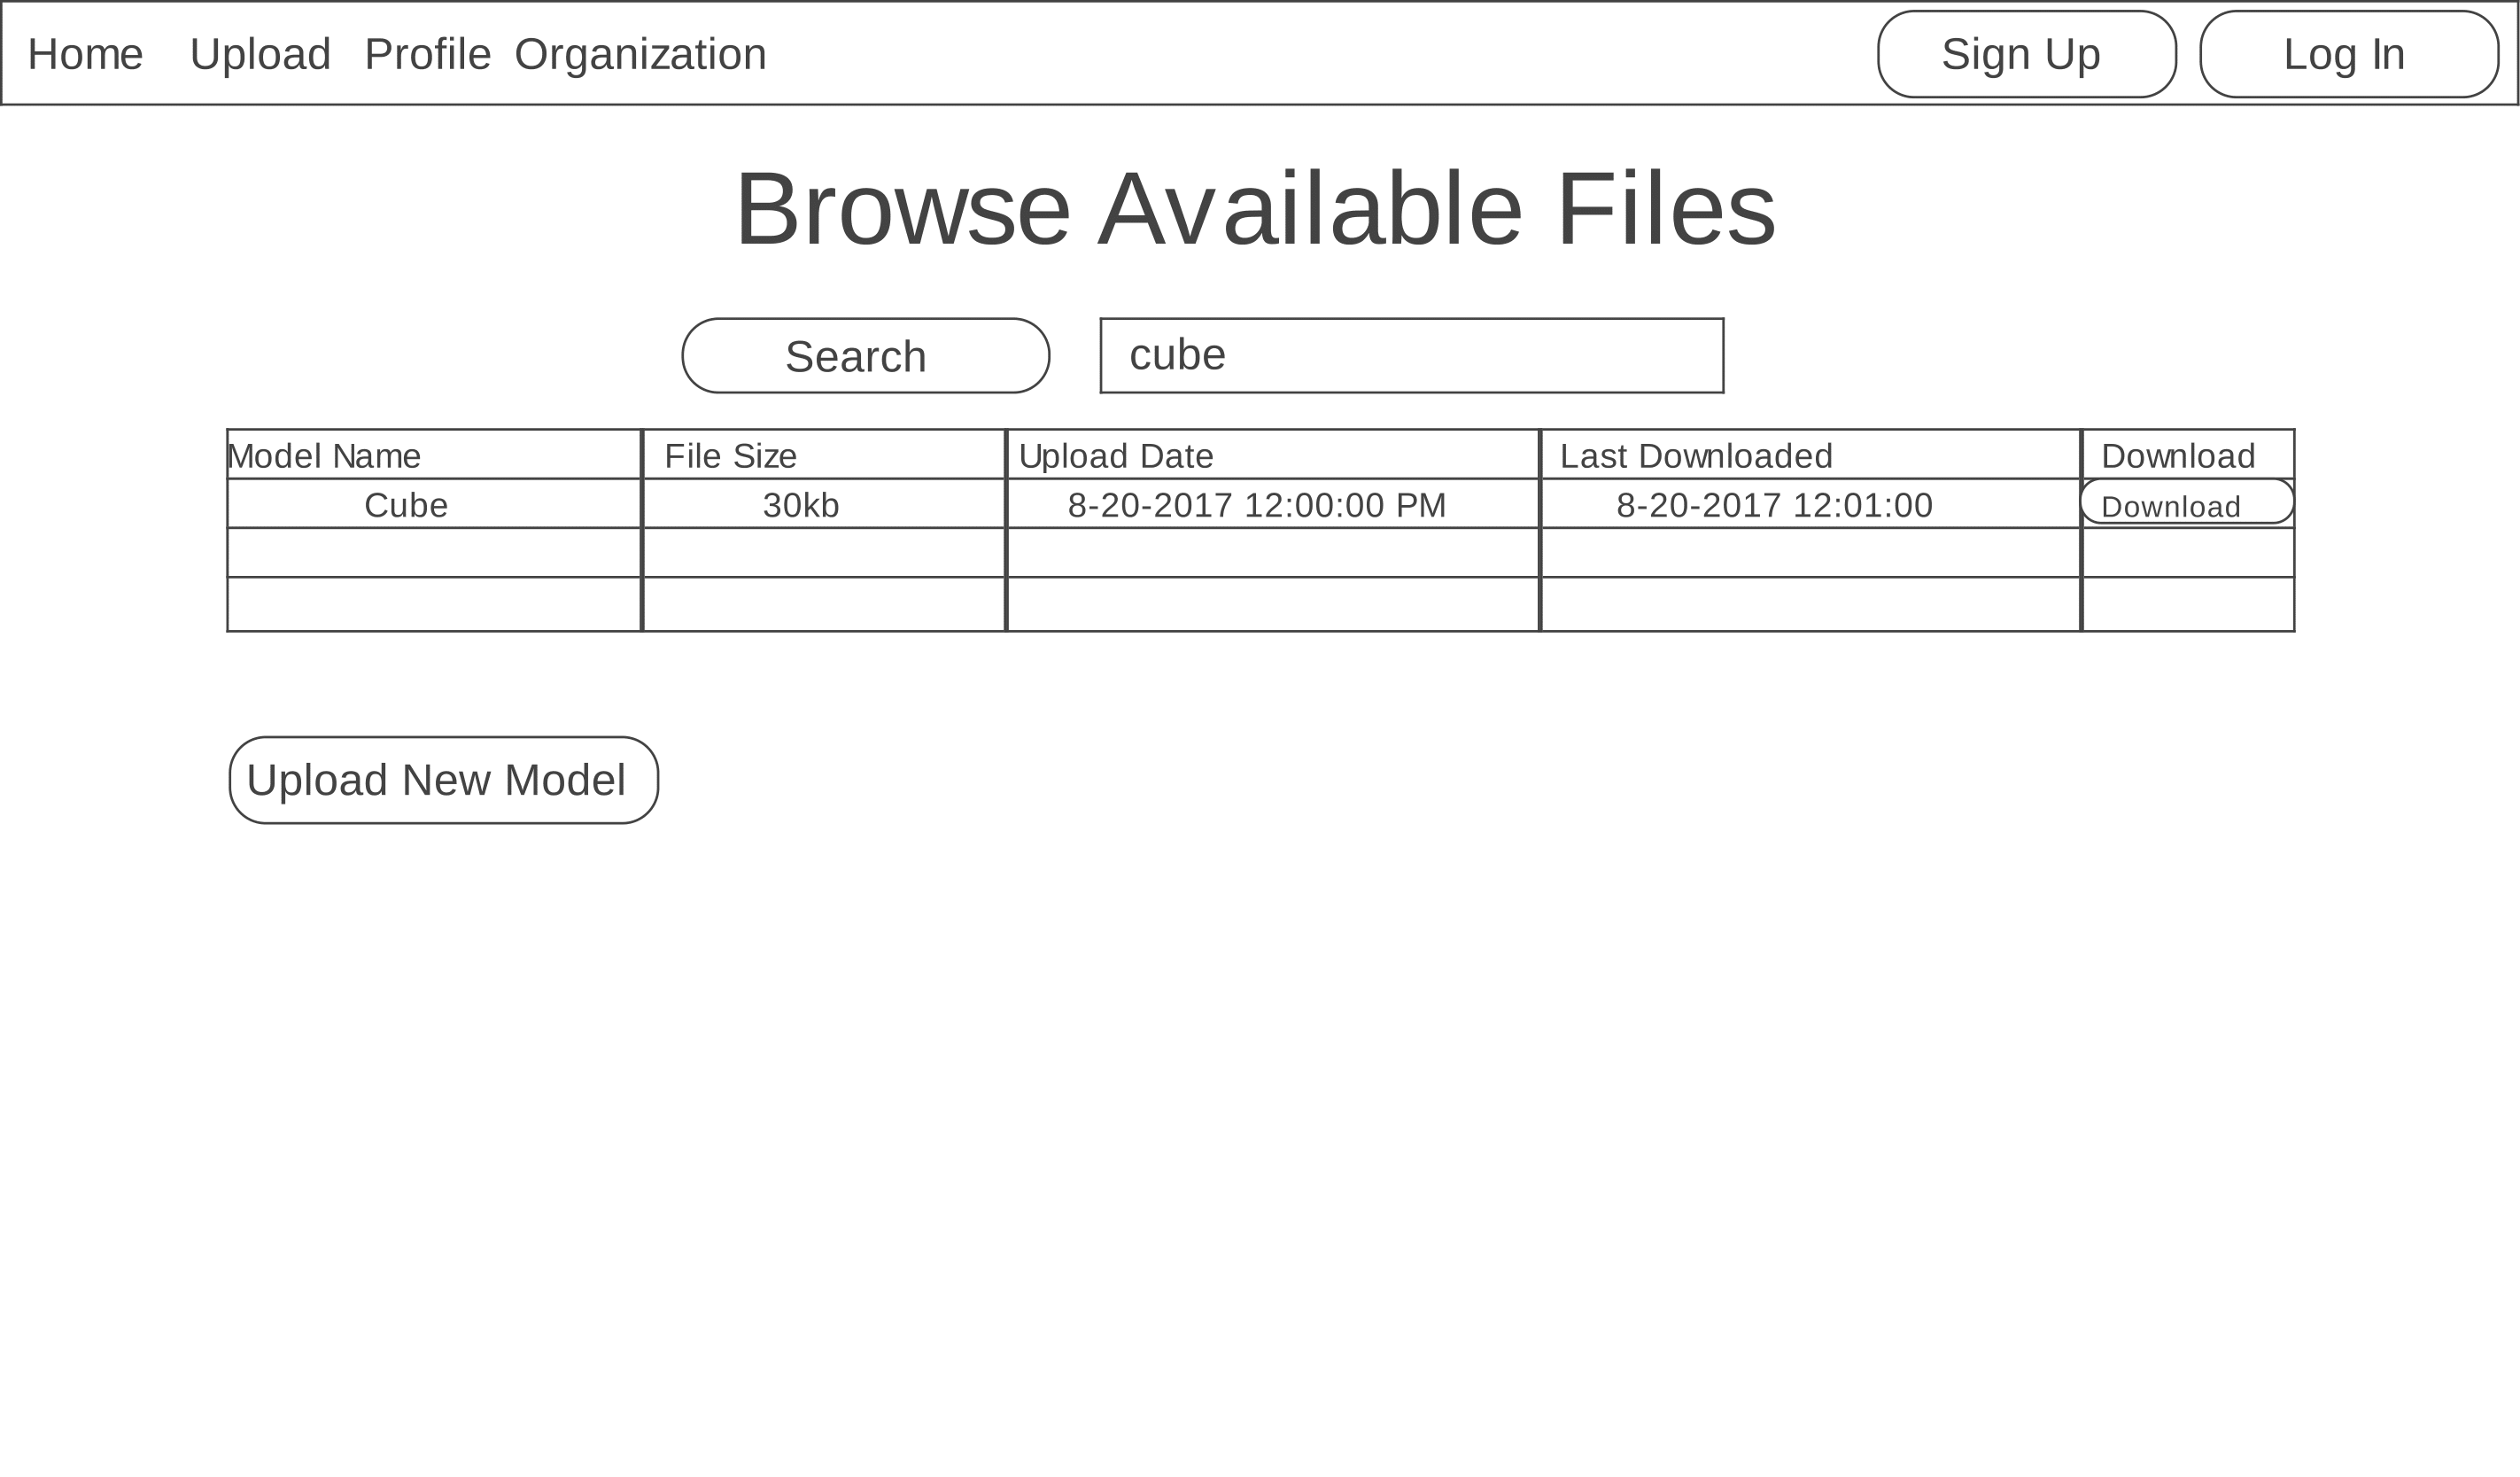
\includegraphics[width=0.6\linewidth]{All}
        \caption{Final design for the Help page}
    \end{figure}
